\clearpage

\section{Marcos do Projeto/Metodologia}

\subsection{Roadmap}

\begin{figure}[h]
    \centering
    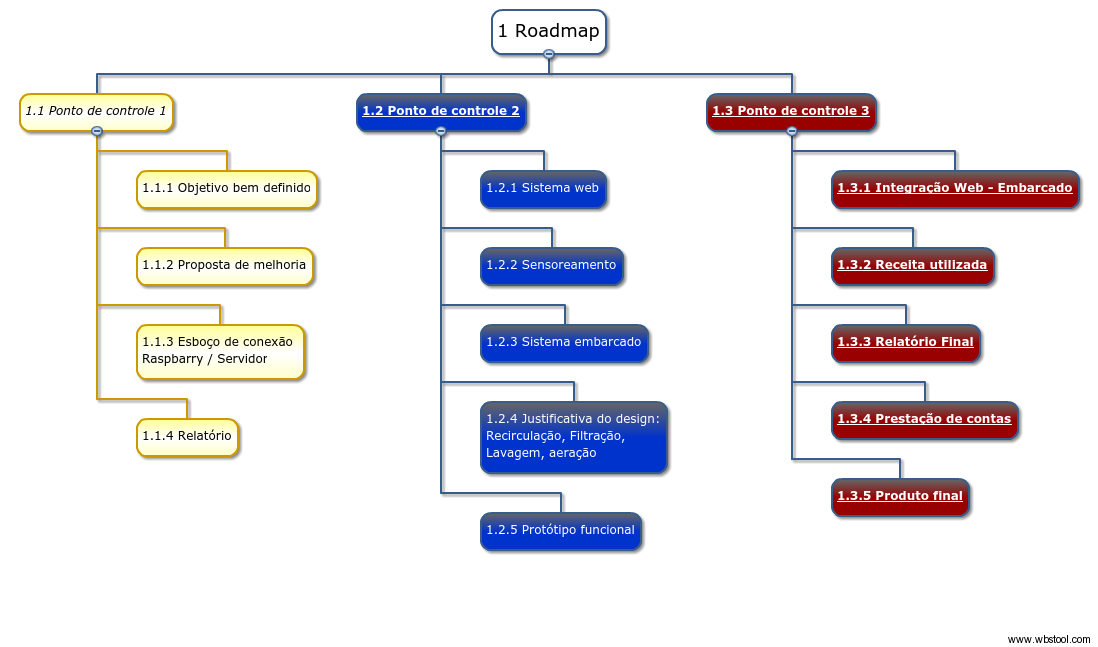
\includegraphics[scale=0.4]{images/pi2-roadmap.png}
    \caption{Roadmap do projeto}
\end{figure}


\subsection{Metodologia de Trabalho}
A equipe de projeto possui 14 membros de 4 engenharias distintas, representando um desafio estratégico para definição de um escopo que integre as 4 áreas e seja corretamente encaminhado, de forma que viabilize a qualidade do trabalho, do produto e não sobrecarregue nenhum dos integrantes em suas áreas de atuação.

Para cumprir esse propósito, o grupo buscou no planejamento de projeto definido pelo PMBOK boas práticas para conduzir o trabalho, e nos princípios ágeis a coordenação da equipe com objetivos claros de circular o conhecimento entre as áreas. Foram feitos alguns dos planos de gerenciamento adotados pelo PMBOK, que se adequavam ao perfil da equipe e no contexto do projeto.

\subsubsection{Comunicação}

O plano de comunicação foi discutido na primeira reunião oficial da equipe. Foi estipulada uma reunião semanal de alinhamento nas quartas-feiras, das 16h às 18h, horário de aula da disciplina Projeto Integrador 2. Nessa reunião as decisões seriam tomadas e foi adotada uma técnica para fazer o conhecimento entre os grupos circular. Nesse espaço de tempo, cada membro do projeto pode explicar o que produziu e indicar para os demais suas restrições.

Para a comunicação casual, e diária, foi escolhida a princípio o whats app, porém, após a primeira semana de trabalho, foi sugerido ao grupo o uso de uma ferramenta com recursos mais profissionais devido a algumas necessidades em relação a divisão de grupos de trabalho e integração com outras ferramentas utilizadas pelo grupo, o que nos levou a escolha da ferramenta de mensagens instantâneas Slack que oferece, além da comunicação em tempo real, um ambiente propício para o trabalho em equipe, colaboração e integração com diversas ferramentas tais como Trello e Google Drive que também são utilizadas pelo grupo.

O grupo ainda está tentando se adaptar a ferramenta, porém, o whats app, por ser uma ferramenta conhecida e comumente usada por todos os integrantes do grupo, continua sendo mais frequente durante a comunicação do grupo referente aos assuntos do projeto. Devido a essas circunstâncias e ao fato de o grupo estar mostrando um bom desempenho, o whats app continua sendo a ferramenta oficial de comunicação dentro da equipe.

\subsubsection{Tempo}

O tempo limite para término do projeto e entrega da solução é o final do semestre e da disciplina ao qual o projeto está inserido. Neste meio tempo, existem duas entregas intermediárias que são encaradas como marcos do projeto, totalizando assim 3 entregas. As atividades e distribuição de trabalho serão baseados nos marcos definidos, ainda que eles não possuam data definida, o grupo trabalha com as estimativas fornecidas pelos professores/orientadores da disciplina.

Para que o as entregas do projeto definidas para cada marco sejam entregues dentro do prazo, o grupo se baseou na metodologia ágil de desenvolvimento denominada Scrum, com algumas adaptações.

\begin{figure}[h]
    \centering
    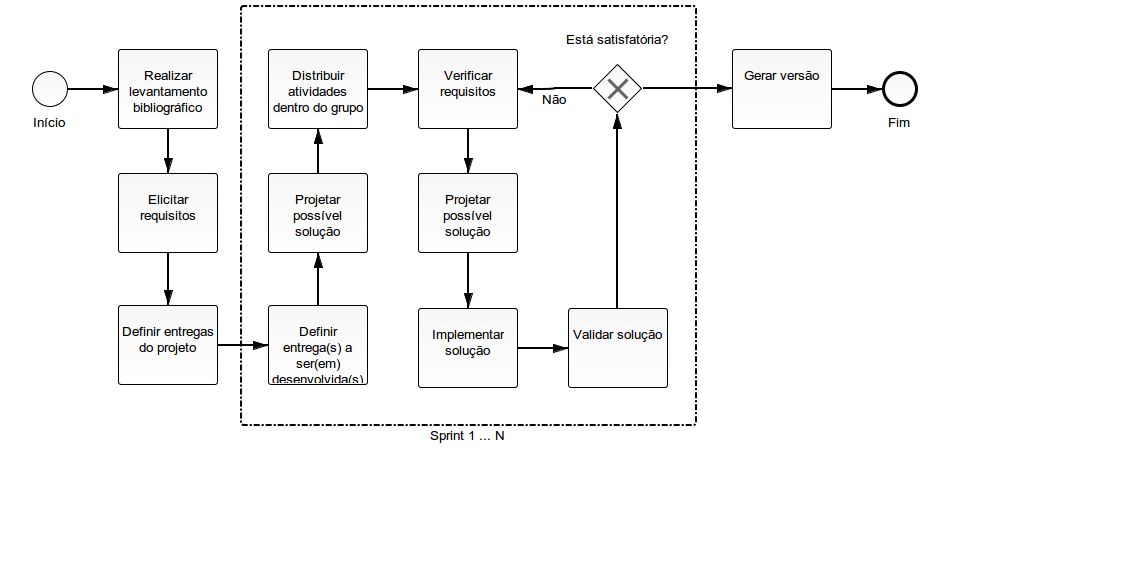
\includegraphics[scale=0.5]{images/pi2-diagram.png}
    \caption{Estruturação de Sprints}
\end{figure}